\chapter{Réalisation et mise en œuvre}

\section*{Introduction}
Dans ce chapitre, nous présentons les environnements matériel et logiciel utilisés,
l’architecture de la solution et nous allons donner un aperçu sur le travail réalisé ainsi
que le résultat de l'integration du module de diagnostic intelligent et recommandation.

\section{Étude Technique}
Dans la présente section, nous allons décrire l’environnent matériel et logiciel utilisé.
    \subsection{Environnement matériel}
    Ce projet a été réalisé à l’aide de trois ordinateurs dont les caractéristiques sont détaillées dans
le \autoref{tab:env_materiel}.

        \begin{table}[H]
        \centering
        \begin{tabular}{|l|l|l|l|}
        \hline
        \textbf{} & \textbf{Processeur} & \textbf{RAM} & \textbf{Système d'exploitation} \\
        \hline
        PC 1 & Intel CORE i7 (13ème génération) & 24 Go & Windows 11 \\
        \hline
        PC 2 & Intel CORE i3 (11ème génération) & 16 Go & Windows 11 \\
        \hline
        PC 3 & Intel CORE i7 (11ème génération) & 8 Go & Windows 10 \\
        \hline
        \end{tabular}
        \caption{Environnement matériel}
        \label{tab:env_materiel}
        \end{table}
    \subsection{Environnement logiciel}

Pour mener à bien notre projet, nous avons utilisé divers logiciels à différentes étapes de sa
réalisation, comme présenté dans le \autoref{tab:env_logiciel}.

        \begin{table}[H]
        \centering
        \begin{tabular}{|p{3cm}|p{3cm}|p{8cm}|}
        \hline
        \textbf{Logiciel} & \textbf{Logo} & \textbf{Description} \\
        \hline
        IntelliJ IDEA & 
        
\includegraphics[width=2cm]{logos/intellij.jpg} & 
        IntelliJ IDEA est un environnement de développement intégré (IDE) développé par JetBrains, reconnu pour ses fonctionnalités avancées d'analyse de code et de complétion intelligente. Il supporte de nombreux langages de programmation et frameworks, ce qui en fait un outil de choix pour le développement d'applications modernes \cite{intellij2011most}. \\
        \hline
        PyCharm & 
        
\includegraphics[width=2cm]{logos/pycharm.jpg} & 
        PyCharm est un IDE spécialisé pour le développement Python, également développé par JetBrains. Il offre des fonctionnalités telles que le débogage, les tests unitaires, et l'intégration avec des frameworks web comme Django et Flask, facilitant ainsi le développement d'applications Python \cite{hu2018deepgraph}. \\
        \hline
        PostgreSQL & 
        
\includegraphics[width=2cm]{logos/postgresql.png} & 
        PostgreSQL est un système de gestion de bases de données relationnelles-objet open source, reconnu pour sa robustesse, sa fiabilité et ses performances. Il supporte des fonctionnalités avancées telles que les transactions ACID, les index partiels et les types de données personnalisés, ce qui en fait l'un des SGBD les plus utilisés dans les applications d'entreprise \cite{postgresql1996postgresql}. \\
        \hline
        OpenAI API & 
        
\includegraphics[width=2cm]{logos/openai.png} & 
        L'API OpenAI fournit un accès aux modèles de langage de grande taille (LLM) développés par OpenAI, notamment GPT-4. Elle permet aux développeurs d'intégrer des capacités d'intelligence artificielle avancées dans leurs applications, telles que la génération de texte, la compréhension du langage naturel et la résolution de problèmes complexes \cite{paredes2023chatgpt}. \\
        \hline
        \end{tabular}
        \caption{Environnement logiciel}
        \label{tab:env_logiciel}
        \end{table}

\section{Travail réalisé}
La figure \ref{fig:arch} illustre l'architecture globale de notre solution, 
ainsi que les technologies et langages de programmation utilisés. Notre architecture 
suit un modèle \textbf{quatre-tiers}, organisé comme suit :

\begin{itemize}
    \item \textbf{Tiers 1 - Couche Présentation (Flutter)} : Le frontend est 
    développé avec le framework Flutter, qui assure l'interface utilisateur de 
    l'application mobile. Il communique avec le backend via des requêtes HTTP 
    en suivant les principes de l'architecture REST. Flutter envoie des requêtes 
    et reçoit des réponses au format JSON, qu'il traite et affiche à l'utilisateur 
    de manière intuitive et réactive.

    \item \textbf{Tiers 2 - Couche Logique Métier (Spring Boot)} : Le backend est 
    développé avec le framework Spring Boot, qui joue le rôle de serveur principal 
    de l'application. Il gère l'ensemble de la logique métier et le traitement des 
    requêtes HTTP provenant du frontend. Spring Boot communique d'un côté avec la 
    base de données PostgreSQL pour assurer la persistance et la récupération des 
    données, et de l'autre côté avec l'API Flask pour les fonctionnalités de 
    diagnostic et de recommandation de plantes.

    \item \textbf{Tiers 3 - Couche Intelligence Artificielle (Flask API)} : L'API 
    Flask constitue le moteur d'intelligence artificielle de notre solution. Elle 
    expose des endpoints REST qui reçoivent les données transmises par Spring Boot, 
    les traitent à l'aide des modèles d'apprentissage automatique intégrés, et 
    retournent les résultats du diagnostic des plantes ainsi que les recommandations 
    appropriées.

    \item \textbf{Tiers 4 - Couche Données (PostgreSQL)} : PostgreSQL assure la 
    persistance et la gestion des données de l'application. Il communique 
    directement avec Spring Boot pour stocker et récupérer l'ensemble des 
    informations relatives aux utilisateurs, aux dossiers médicaux, aux 
    consultations et aux plantes médicinales.
\end{itemize}

    La \autoref{fig:arch} est une capture d'écran de Bloomscape.
    \subsection{Architecture globale de la solution}
        \begin{figure}[H]
        \centering
        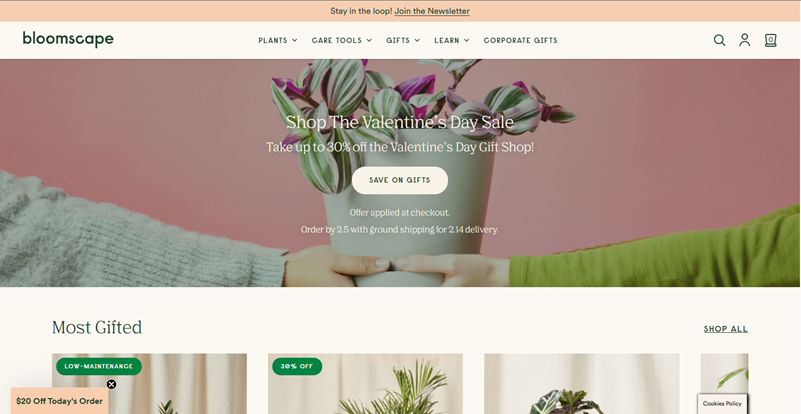
\includegraphics[width=0.6\textheight]{images/bloomscape.png}
        \caption{ Capture d'écran de la page accueil de BloomscapeRef1 \cite{BloomscapeRef1}.}
        \label{fig:arch}
        \end{figure}

    \subsection{Aperçu sur le travail réalisé}
Dans cette partie, nous décrivons les différentes interfaces de notre plate-forme, PhytoCare

        \subsubsection{La page de connexion (SignIn)}
        ...

        \subsubsection{La page d'inscription (Sign Up)}
        ...
        \subsubsection{La page d'accueil}
        ...
        \subsubsection{La page panier}
        ...

        \subsubsection{La page dianostic}
        ...


\section*{Conclusion}
Ce chapitre final a été consacré à la présentation des résultats de notre travail 
réalisé sur notre application PhytoCare, en décrivant les environnements matériel 
et logiciel utilisés, l'architecture, ainsi que quelques interfaces de la plateforme.